\chapter{Asking Dubai Billionaires How They Got Rich}

This lecture begins with spectacle, but it does not stay there. The opening splice gives us yachts, Rolls-Royces, and billionaire-sized yearly numbers before any stable explanation arrives, and then the host resets the scene and begins the real work: a sequence of interviews in Dubai that move from risk, to sales, to brokerage arithmetic, to product design, and finally to focus and faith. What makes the chapter worth writing carefully is that the lecture does not merely stack anecdotes; it repeatedly turns anecdotes into small operator rules, and those rules can be written down with some discipline.

\section{Cold Open and the Dubai Field Site}

The first forty seconds are a teaser reel. We are shown the endpoint first: a yacht, giant annual figures, the phrase ``first billionaire from cannabis,'' six Rolls-Royces, and a blunt question about how one owns a yacht in the present world. We should preserve that rhythm, because it is part of the lecture's method. First the result, then the mechanism. But we should not treat the cold open as a stable source of arithmetic. The later interviews are cleaner.

After this splice, the host resets everything. He tells us where we are, why we are there, and what the viewer is supposed to extract from the episode: not simply admiration, but a copyable blueprint. In that sense the lecture is a field study in several business doctrines rather than a single autobiography. The sequence is deliberate: cannabis and risk first, yacht wealth and pivot second, real-estate entry arithmetic third, and developer-scale branding and focus last.

We can summarize the opening tension in one line:
\begin{equation}
\text{visible wealth} \to \text{hidden mechanism?}
\end{equation}
The rest of the lecture is an attempt to fill in the right-hand side.

\section{Cannabis, Risk, and Leverage}

The first full interview settles on the cannabis billionaire. The lecture first establishes scale, because it wants authority before doctrine:
\begin{equation}
Y_{\text{cannabis}} \approx 1\,\text{billion euros/year}.
\end{equation}
But the number is not the only point. The lecture immediately asks what kind of advice sits behind such scale, and the answer is a father's rule about recoverable risk:
\begin{equation}
10 \to 20,
\qquad
\text{because }10\text{ can be earned again.}
\end{equation}
We should read this as a heuristic, not as a finance theorem. The right abstraction is simply
\begin{equation}
\text{recoverable downside} \to \text{willingness to risk for larger upside}.
\end{equation}
That is the lecture's first real operator identity.

The guest then gives the first cautionary business lesson: giant success does not erase exposure. He says he had been broke several times, and not even very long ago lost his money in the Cyprus banking crisis. From that comes a deliberately sharp claim:
\begin{equation}
\text{money in the bank} \neq \text{money under direct control}.
\end{equation}
A cautious schematic rendering is
\begin{equation}
D_{\text{customer}} \mapsto L_{\text{bank}},
\end{equation}
meaning that once a deposit enters the bank, what we directly possess is a claim on the institution, not a stack of notes in a private drawer. The lecture does not present a full banking theory, and we should not pretend otherwise, but it does insist that banked money is not equivalent to perfectly controlled money.

From here the interview pivots into social environment. The speaker's proverb is coarse but mathematically clean enough to preserve:
\begin{equation}
n_{\text{drunks}}=5 \to \text{you become the 6th drunk},
\qquad
n_{\text{billionaires}}=5 \to \text{you become the 6th billionaire}.
\end{equation}
In more abstract form,
\begin{equation}
\text{peer group} \to \text{behavioral drift} \to \text{identity outcome}.
\end{equation}
This then prepares the lecture's motivational distinction between the billionaire and the millionaire:
\begin{equation}
\text{work} \to \text{success},
\qquad
\text{not primarily } \text{work} \to \text{money}.
\end{equation}
The idea is not that money is absent, but that money is treated as the byproduct of a larger target.

The interview closes with a memorable hard line: ``don't negotiate.'' The host interprets that for us, and we should preserve the interpretation rather than only the swagger:
\begin{equation}
\text{leverage}\uparrow \to \text{need to negotiate}\downarrow,
\qquad
\text{walk-away power}\uparrow.
\end{equation}

\subsection{Question \& Answer}

\paragraph{Question.} What changes when leverage is strong enough that one can walk away instead of negotiate?

\paragraph{Answer.} The lecture's answer is that bargaining ceases to be the central skill. If the operator can live without the deal, then the deal must fit the operator rather than rescue him. ``My way or the highway'' is therefore not merely personality. It is the practical surface of walk-away power.

\section{Yacht Wealth and the COVID Pivot}

The lecture then changes scene and changes the kind of problem. At Dubai Harbor, the host goes after owners of multimillion-dollar yachts, and the new interview turns from abstract billionaire identity toward a very specific scaling story. Here the clean numbers are
\begin{align}
R_{\text{pre-pivot}} &\approx \$10\,\text{million}, \\
R_{\text{pivot-year}} &\approx \$69\,\text{million}, \\
R_{\text{core,later}} &\approx \$35\,\text{million}.
\end{align}
The operator says his whole business crashed during COVID, that exhibitions closed, and that promotional products stopped moving. That is the negative impulse. The positive response is a pivot: medical supplies, operational knowledge in China, and direct sales to hospitals. Schematically,
\begin{equation}
\text{promotional products crash}
\to
\text{medical supplies pivot}
\to
\text{direct hospital sales}
\to
R_{\text{pivot-year}}.
\end{equation}

\begin{figure}[h]
\centering
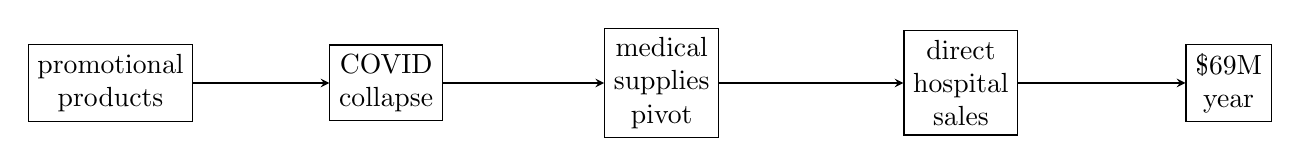
\begin{tikzpicture}[>=stealth]
\node[draw, align=center] (a) at (0,0) {promotional\\products};
\node[draw, align=center] (b) at (3.5,0) {COVID\\collapse};
\node[draw, align=center] (c) at (7.0,0) {medical\\supplies\\pivot};
\node[draw, align=center] (d) at (10.8,0) {direct\\hospital\\sales};
\node[draw, align=center] (e) at (14.2,0) {\$69M\\year};

\draw[->] (a) -- (b);
\draw[->] (b) -- (c);
\draw[->] (c) -- (d);
\draw[->] (d) -- (e);
\end{tikzpicture}
\caption{Editorial reconstruction of the lecture's pivot mechanism: the crisis matters, but only because it forces a change of product and sales channel.}
\end{figure}

There is also a small arithmetic tension here, and the notes should not hide it. If we compute the host-framed jump directly, we obtain
\begin{equation}
g_{\text{pivot}}
=
\frac{R_{\text{pivot-year}}}{R_{\text{pre-pivot}}}
\approx
\frac{69}{10}
\approx 6.9.
\end{equation}
But the guest later says ``5x the business before.'' The safe thing to do is to preserve both statements and note the mismatch rather than harmonize them artificially.

\subsection{Question \& Answer}

\paragraph{Question.} How do we pivot when the original business collapses?

\paragraph{Answer.} In the lecture, a pivot is not a mood shift. It is the conjunction of three things: a new urgent product, an existing operational competence that can support it, and a new sales path that reaches the buyer directly. Crisis by itself does not produce growth. Crisis plus a usable channel does.

\section{Sales as Question-Removal}

Once the pivot is on the table, the lecture naturally turns into a sales seminar. The guest says this repeatedly enough that it deserves to be preserved nearly verbatim:
\begin{equation}
\text{selling was key before},
\quad
\text{selling is key today},
\quad
\text{selling will be key in the future}.
\end{equation}
This is not a side remark. It is the bridge from business history to business method.

The lecture's most useful formalization here is a closing model. The guest says the secret is to ask so many questions that the customer would be foolish not to buy afterward. We can render that carefully as
\begin{equation}
Q\uparrow \to O\downarrow \to P(\text{close})\uparrow,
\end{equation}
where \(Q\) is useful questioning, \(O\) unresolved objections, and \(P(\text{close})\) the probability of closing. The underrated question he names is especially telling: ask the prospect what he liked most about the presentation. Then keep digging: what else? what else? The point is to make the customer state the value structure out loud, which is a cleaner close than pushing prematurely.

The lecture then adds another piece that is easy to miss if we moralize sales too quickly: payment friction matters. The guest says that roughly \(80\%\) of customers usually pay with a named card path, and the larger doctrine is
\begin{equation}
p_{\text{card XYZ}} \approx 0.8,
\qquad
\text{payment friction}\downarrow \to P(\text{pay})\uparrow.
\end{equation}
Closing is not only persuasion. It is also the removal of procedural difficulty.

\subsection{Question \& Answer}

\paragraph{Question.} What question actually moves a sale toward closure?

\paragraph{Answer.} The lecture's answer is not a magic closing line but a way of extracting the customer's own positive criteria. ``What did you like most?'' works because the buyer begins to explain the offer back to himself. Once that happens, objection handling becomes cleaner, because the conversation has shifted from pressure to clarification.

\section{Mindset, Self-Direction, and the Profitable Belief}

The harbor interview then widens from sales technique to entrepreneurial psychology. The guest says that \emph{Think and Grow Rich} mattered to him, but the form in which the lesson survives in the lecture is this:
\begin{equation}
S_{\text{entrepreneurship}} \approx 0.9\,\text{mindset}+0.1\,\text{financial technique}.
\end{equation}
We should keep this with a firm caveat: it is a heuristic slogan, not a measured decomposition. Still, it matters because it tells us what the lecture thinks technique sits on top of.

The self-talk doctrine later sharpens the same point:
\begin{equation}
\text{words to oneself} \to \text{subconscious response} \to \text{action}.
\end{equation}
Here belief is not merely decorative. The guest says that even when one feels bad, one should speak health and strength to oneself, because the mind follows the words. The host's recap then distills the lesson into an economic sentence: believing that one can is more profitable than believing that one cannot. That is not rigorous psychology, but it is rigorous enough as the lecture's operating assumption.

We should also notice the structure of this transition. The lecture first teaches closing mechanics, then tells us that even those mechanics depend on inner direction. The notes ought to preserve this order. If we reverse it, we turn an operating lecture into a motivational tract.

\section{Real Estate Without Starting Capital}

The next interview begins by clearing a familiar obstacle. The guest says one does not need inherited money in order to become a billionaire, and offers the headline figure
\begin{equation}
p_{\text{first-gen billionaires}} \approx 0.85.
\end{equation}
The second-generation follow-up number is too garbled to stabilize, so we leave it alone. What matters is the lecture's decision to remove the inheritance objection before giving the arithmetic.

Only then does the clearest numerical example of the lecture appear. The guest says that if one lacks capital and wants to enter real estate, one should begin in brokerage. In Dubai, he says, the commission is about \(5\%\). On a \(10\)-million-dirham property, the arithmetic is immediate:
\begin{align}
c_{\text{broker}} &= 5\%, \\
V &= 10\,\text{million AED}, \\
c_{\text{broker}}V &= 0.5\,\text{million AED}.
\end{align}
This deserves to be written out as a worked example.

\paragraph{Worked Example.}
\begin{enumerate}
\item Take the commission rate \(c_{\text{broker}}=5\%=0.05\).
\item Take the transaction size \(V=10{,}000{,}000\ \text{AED}\).
\item Multiply:
\[
0.05 \times 10{,}000{,}000 = 500{,}000.
\]
\item Therefore the broker's commission is
\[
c_{\text{broker}}V = 500{,}000\ \text{AED} = 0.5\,\text{million AED}.
\]
\end{enumerate}
The lecture's ladder is then simple:
\begin{equation}
\text{brokerage} \to \text{developer}.
\end{equation}
One begins with the commission machine, then climbs into ownership and development.

The same interview then returns to sales, but now with real-estate specificity. The guest insists that a good salesperson must first understand the customer's requirement, available money, and appetite for luxury or affordability. A compact summary is
\begin{equation}
\text{buyer need} + \text{budget fit} + \text{ROI clarity}
\to
P(\text{purchase})\uparrow.
\end{equation}
The language around speed of return is rough in the transcript, but the underlying point is clear: a property sale closes more easily when the buyer can see not only what the asset is, but what it will do for his money.

\subsection{Question \& Answer}

\paragraph{Question.} How can somebody start creating wealth in real estate today if he does not begin with capital?

\paragraph{Answer.} The lecture's answer is to begin where transaction size already exists but ownership is not yet required. Brokerage is valuable because the asset belongs to someone else while the commission can belong to us. The operator uses distribution first, capital accumulation second, and only afterward moves toward development.

\section{Product, Omnipresence, One Core, and Faith}

After the sponsor hinge, the lecture returns at a higher altitude with a property developer. Again it begins with scale:
\begin{equation}
Y_{\text{developer}} \approx \$5\,\text{billion}/\text{year}.
\end{equation}
But immediately the guest translates scale into method: sales and marketing are everything. The more subtle claim follows a moment later. The goal of marketing is not merely attention in the short run. It is omnipresence:
\begin{equation}
\text{marketing} \to \text{omnipresence}.
\end{equation}
And the way he claims to have approached that, especially with limited early resources, is to let the product itself function as the visibility engine.

This is one of the chapter's most useful abstractions:
\begin{equation}
\text{architectural DNA}
\to
\text{recognizability}
\to
\text{self-marketing product}.
\end{equation}
The buildings become the billboards. The operator does not merely buy visibility; he bakes visibility into the object.

\begin{figure}[h]
\centering
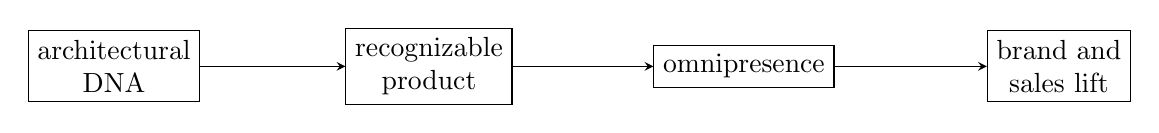
\begin{tikzpicture}[>=stealth]
\node[draw, align=center] (a) at (0,0) {architectural\\DNA};
\node[draw, align=center] (b) at (4,0) {recognizable\\product};
\node[draw, align=center] (c) at (8,0) {omnipresence};
\node[draw, align=center] (d) at (12,0) {brand and\\sales lift};

\draw[->] (a) -- (b);
\draw[->] (b) -- (c);
\draw[->] (c) -- (d);
\end{tikzpicture}
\caption{Editorial reconstruction of the developer's marketing doctrine: the product acquires a visual language, the language creates recognition, and recognition substitutes for part of paid advertising.}
\end{figure}

The lecture then moves to focus. The guest says outright that one of his mistakes had been diversification across unrelated sectors. What finally worked was staying in one core and widening inside it:
\begin{equation}
\text{one core} \to \text{multiple product lines within the core} \to \text{scale}.
\end{equation}
The host summarizes that as vertical integration. This is not vertical integration in the most technical industrial sense, but the approximation is close enough for the lecture's purpose:
\begin{equation}
\text{focus within one core} \approx \text{vertical integration}.
\end{equation}
The important point is not the label. It is the refusal to scatter entrepreneurial energy across unrelated games.

\subsection{Question \& Answer}

\paragraph{Question.} How can the product itself perform part of the marketing?

\paragraph{Answer.} The lecture's answer is that a product can carry a repeated visual grammar, so that recognition arises before explanation. If the building is identifiable in the way a Bugatti is identifiable, then marketing has already begun before a salesperson says a word.

The final movement is faith. The developer says it is everything, speaks of miracles, and recounts a moment when he thought all was lost and asked God to take over where calculation had stopped. We should not over-formalize this. The lecture's point is simply that belief remains one more operating resource when technique seems exhausted. It closes the chapter by suggesting that focus and sales build the machine, but hope keeps the operator in motion when the machine stalls.

\section{Summary}

The lecture begins with display and ends with discipline. First it shows us yachts, billionaires, and giant yearly numbers. Then it asks what sort of operator rules can sit underneath such surfaces. The answers come in a definite order: risk what can be re-earned, do not confuse a bank deposit with direct control, let peer groups shape ambition upward rather than downward, turn walk-away power into leverage, pivot fast when the old channel collapses, treat sales as the removal of objections rather than mere pressure, use brokerage as a low-capital entry into real estate, and let the product itself become part of the marketing engine.

What remains after the episode is not one doctrine but a chain:
\begin{align}
\text{recoverable downside} &\to \text{risk}, \\
\text{pivot} &\to \text{new channel}, \\
Q\uparrow &\to O\downarrow \to P(\text{close})\uparrow, \\
\text{brokerage} &\to \text{developer}, \\
\text{architectural DNA} &\to \text{recognizability} \to \text{omnipresence}, \\
\text{one core} &\to \text{scale}.
\end{align}
The lecture is therefore most useful when read not as a gallery of rich people, but as a layered study in how risk, sales, positioning, and belief fit together into a commercial life.